\documentclass[notes]{beamer}
\usepackage[english]{babel}
\usepackage[utf8]{inputenc}
\usepackage{tcolorbox}

\usetheme{ENSLyon}

\title[Title]{Dicotomix}
\author[T.S]{M. Guy, E. Hazard, E. Kerinec, F. Lecuyer, P. Mangold,\\ A. Martin, R. Pellerin, N. Pinson, A. Slowik, T. Stérin}
\date{\today}

\setbeamersize{text margin left=20pt,text margin right=20pt}
\setbeamertemplate{navigation symbols}{}
\usecolortheme{ENSLyon_blue}
\addtobeamertemplate{navigation symbols}{}{
	\usebeamerfont{footline}
	\usebeamercolor[fg]{footline}
	\hspace{1em}
	\insertframenumber/\inserttotalframenumber
}

\begin{document}

\begin{frame}
	\titlepage
	\begin{center}
		
\includegraphics[scale=0.2]{dicotomix}
		
\includegraphics[scale=0.08]{logoens}
		\hspace{2em}
		
\includegraphics[scale=0.55]{ars}
		\hspace{2em}
		
\includegraphics[scale=0.3]{hospices_civils_de_lyon}
	\end{center}
\end{frame}

\section*{Content}
\begin{frame}
	\tableofcontents
\end{frame}

\section{Introduction}
\subsection{Motivations}

\begin{frame}{Charcot disease and locked-in syndrome}
	\begin{center}
		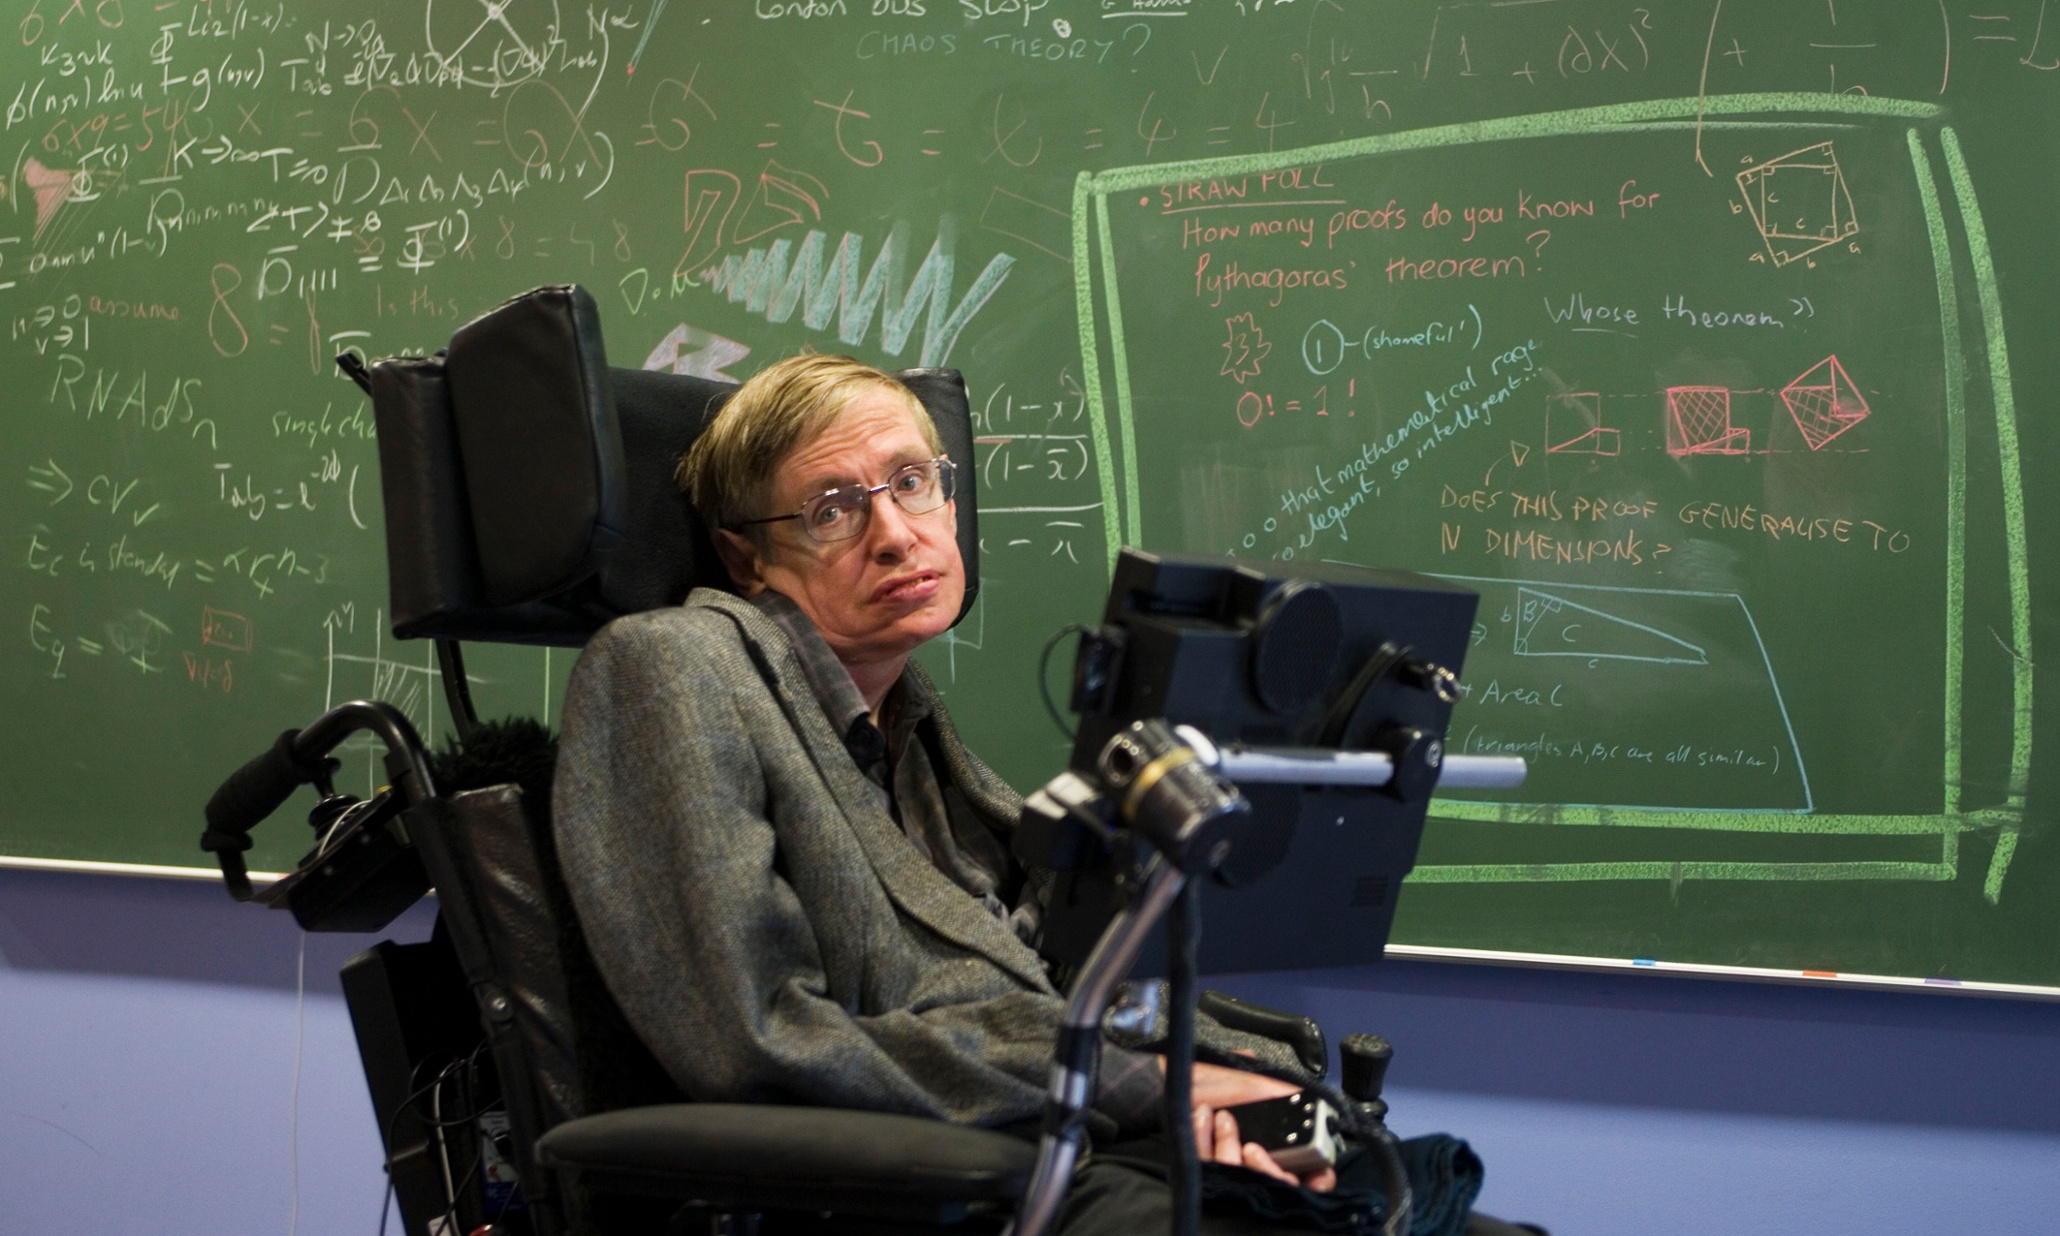
\includegraphics[scale=0.5]{hawking}
	\end{center}
\end{frame}

\begin{frame}{Charcot disease and locked-in syndrome 2}
	\begin{center}
		\begin{itemize}
			\item Almost entirely paralized
			\item Keeping all cognitive abilities
		\end{itemize}
	\end{center}
\end{frame}

\begin{frame}{Existing methods : EJASINT}
	\begin{center}
		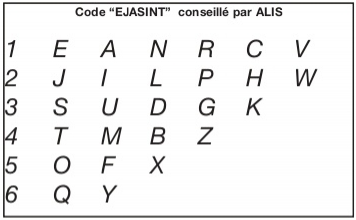
\includegraphics[scale=0.7]{ejasint}
	\end{center}
\end{frame}

\begin{frame}{Existing methods : ARS}
	\begin{center}
		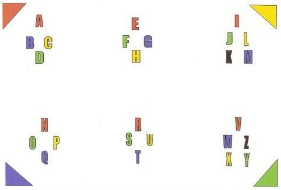
\includegraphics[scale=0.9]{tableau_lettres_transparent}
	\end{center}
\end{frame}

\begin{frame}{Existing methods : "Par-Lé-Si-Lab"}
	\begin{center}
		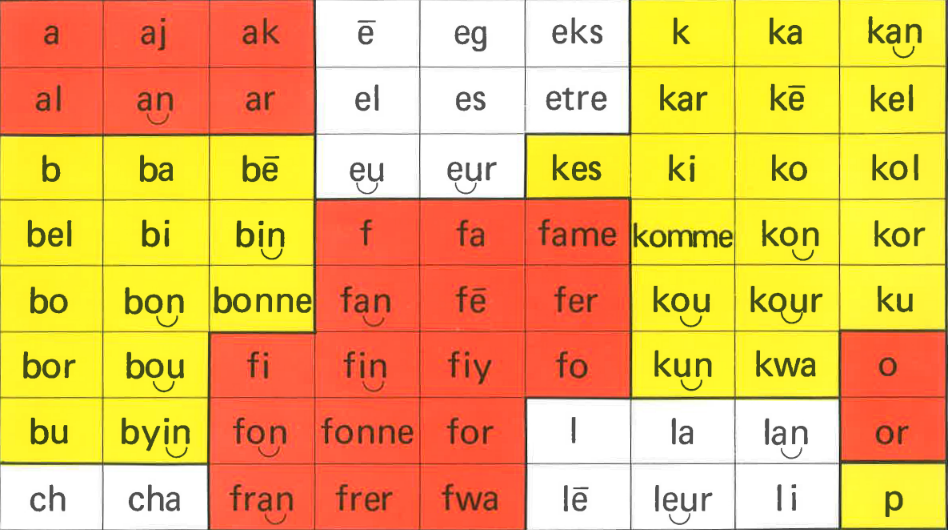
\includegraphics[scale=0.3]{parler_syllabes}
	\end{center}
\end{frame}

\note[itemize]{
	\item bob
	\item alice
}
\subsection{Dicotomix idea}
\begin{frame}{Concept}
	\begin{center}
		\begin{itemize}
			\item Write word by word rather than spelling
			\item Optimize every question
			\item Intuitive thanks to a simple interface
			\item The only requirement is a binary input
		\end{itemize}
	\end{center}
\end{frame}

\section{Dicotomix method}
\subsection{Algortithm}
\begin{frame}{Algorithm}
	\begin{center}
		\begin{itemize}
			\item Dicotomy over a dictionary (right/left signals)
			\item Frequences of words taken into account
			%plus tard gestion dynamique fréquences
		\end{itemize}
	\end{center}
\end{frame}

\subsection{Demo}
\begin{frame}{Demo}
	\begin{center}
		%DEMO!
	\end{center}
\end{frame}

\begin{frame}{Assets / Drawbacks}
	\begin{tcolorbox}[colback=green!5,colframe=green!40!black,title=A nice heading]
		
	\end{tcolorbox}
\end{frame}

\begin{frame}{Modularity}
	\begin{center}
		\begin{itemize}
			\item Use of every possible dictionary %ajout de mots
			\item Possibility to change frequencies using some heuristics
			\item Adaptation to the patient
		\end{itemize}
	\end{center}
\end{frame}

\section{Demarche}
\subsection{Contacts}
\begin{frame}{Contacts}
	\begin{center}
		%graphe de Fabrice (mettre à jour) -> ajouter linguistes, métropole de Lyon, (physicien)
		%parler du bullshit?
	\end{center}
\end{frame}

\begin{frame}{Evolutions}
	\begin{center}
		\begin{itemize}
			\item Use of BCI, at the beginning
			\item Ergonomy, cognitive cost %interface simple, intuitive
			\item Modularity (Web interface)
		\end{itemize}
	\end{center}
\end{frame}

\section{In the future}
\subsection{Test phase}
\begin{frame}{Clinical trials}
	\begin{center}
		\begin{itemize}
			\item Hôpital Lyon Nord %à vérifier
			\item a few patients
			\item a training phase and a evaluation phase %décrire le protocole
		\end{itemize}
	\end{center}
\end{frame}

\subsection{Distribution}
\begin{frame}{Reaching patients}
	With the help of: 
	\begin{itemize}
		\item metropole de Lyon
		\item ARSLA
		\item with possibly other partners %citer la meuf qui vient nous voir
	\end{itemize}
\end{frame}

\begin{frame}{Questions ?}
	\begin{center}
		Merci de votre attention
	\end{center}
\end{frame}
\end{document}